\documentclass[12pt]{article}
\usepackage{amsmath}
\usepackage{graphicx}
\usepackage{hyperref}
\usepackage[latin1]{inputenc}
\usepackage[top=2cm, bottom=2cm, left=2cm, right=2cm, headsep=14pt]{geometry}
\usepackage[T1]{fontenc}
\usepackage[utf8]{inputenc}

\title{Report 1}
\author{Group 2}
\date{January 17, 2018}

\begin{document}
\maketitle
  \section{Why we choose our specific MapReduce implementation:}
    In this labwork, we chose Apache Hadoop because it is the most common open-source software framework using MapReduce programming model. Hadoop is also easy to use and there are plenty of instructions that we can follow to learning about it. 
  
  \section{How our Mapper and Reducer work:}
    Mapper takes in 2 inputs: file name (string) and number of lines (integer). It reads the content of the file line by line and takes each word in a line as a key with value of 1. For example, in a line "Hello world from the world", we have <hello, 1>, <world, 1>, <from, 1>, <the, 1>, <world, 1>. \\\
    Reducer adds all the values which are from the same key to produce the occurrence of a word. In the previous example, after pairs of key and value are created by the mapper, there are 2 pairs having the identical key, <world>. The reducer adds the values of these two pair to create <world, 2>.
    \begin{figure}[h]
      \centering
      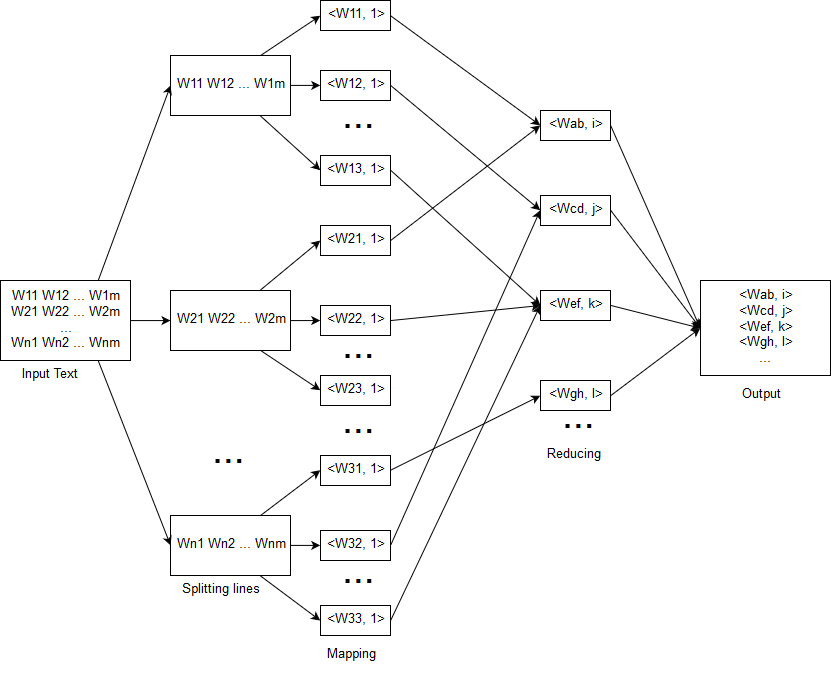
\includegraphics{WordCounter.png}
    \end{figure}

\end{document}